\subsubsection{Time domain analysis}
We showed in section \ref{sec:eff_mass} that we can map the two-dimensional membrane onto a one-dimensional model, by introducing an effective mass. In this chapter we will present some of the general results of the one-dimensional damped harmonic oscillator, which is equivalent to the textbook example of mass a suspended on a spring system. At least for us doing cavity optomechanics. In fact a mirror on a spring is the canonical example of a cavity optomechanical system.

We already considere the solution of the rather dull case of a harmonic oscillator with no damping in chapter \ref{sec:vib_modes}, so we will skip it and jump directly to introducing a viscous damping term $\Gamma_m = b/m$, which is proportional to the velocity $\dot{x}(t)$ (the dot symbolises a time derivative). We can write out the equations of motion of the system

\begin{align}
m\ddot{x}(t) + b\dot{x}(t) + kx(t) &= 0 \\
\ddot{x}(t) + \gamma\dot{x}(t) + \omega_{m,n}^2x(t) &= 0,
\end{align}
\noindent
whit $\Omega_{m} = \sqrt{k/m}$, where $k$ is the spring constant and $m$ the mass. We can easily solve this exactly and show that it is an exponentially decaying cosine, if the damping term is relatively small ($\Omega_{m} \gg \Gamma_m$) \cite{young2003} (see figure \ref{fig:damped_osc})

\begin{equation}
x(t) = x_0e^{-\frac{\gamma}{2}t}\cos(\Omega_0t + \varphi),
\end{equation}
\noindent
where $\Omega_0 = \sqrt{\Omega_{m}^2 - \left(\frac{\Gamma_m}{2}\right)^2}$, $x_0$ is the amplitude and $\varphi$ is the phase. There are three different damping regimes:

\begin{itemize}
\item Underdamped ($\Omega_m > \frac{\Gamma_m}{2}$): The system oscillates with a slightly different frequency, compared to the undamped case, and slowly decays to its resting position (equilibrium).
\item Critically damped ($\Omega_m = \frac{\Gamma_m}{2}$): The system returns to equilibrium as quickly as possible without oscillating.
\item Overdamped ($\Omega_m < \frac{\Gamma_m}{2}$): Returns exponentially to equilibrium without oscillating, but slower for large $\Gamma_m$ and can overshoot the equilibrium position as seen in figure \ref{fig:damped_osc}.
\end{itemize}

\begin{figure}[H]
\centering
\includegraphics[scale=0.6]{damped_oscillator.pdf}
\caption{Behaviour of a damped harmonic oscillator for three different damping coefficients regimes.}
\label{fig:damped_osc}
\end{figure}

The result is a basic result that all physicists should know, but none the less, it is an important result in optomechanics. The $1/e$-time is what defines the ringdown time $\tau = 1/\Gamma_m$, i.e. how quickly energy dissipates from the system when excited. This is used for both cavities and membranes to characterize their dissipation rates. Another example for why this is important, is that membranes could potentially be used as memory, because of their slow decoherence rate.

\subsubsection{Frequency domain analysis}
Another way of solving the equation of motion of a one-dimensional oscillator is by using the Fourier transform. This time we will add an external force $F_{ext}(t)$ to the model and write out the equations of motion. Performing the Fourier transform is a trivial matter since we are dealing with a differential equation ($\frac{d}{dt} \rightarrow -i\Omega$ and $\frac{d^2}{dt^2} \rightarrow -\Omega^2$)

\begin{align}
\left(\ddot{x}(t) + \Gamma_m\dot{x}(t) + \Omega_{m}^2x(t)\right)m & = F_{ext}(t) \\
m\left[-\Omega^2 + \Omega_{m}^2 -i\Omega\Gamma_m\right]x(\Omega) & = \chi(\Omega)^{-1}x(\Omega) = F_{ext}(\Omega),
\end{align}
\noindent
where $\chi(\Omega)$ is the mechanical susceptibility of the system. We will specify the properties of the newly introduced driving force later on. We can easily write the power spectral density of the system using equation \eqref{eq:PSD}, if we assume operation near resonance $\Omega \approx \Omega_{m}$, which means that $\Omega + \Omega_{m} \approx 2\Omega$ and $\Omega/\Omega_{m} \approx 1$, while the detuning (small differences) $\Delta = \Omega_{m} - \Omega$ will still be of interest and not approximated with zero. The power spectral density takes the following form

\begin{equation}
\begin{split}
S_{xx}(\Omega) & = \left|S_{xx}^{ext}(\Omega)\chi(\omega)\right|^2 = \frac{\left|S_{xx}^{ext}(\Omega)\right|^2}{m}\left[(\Omega_{m}^2 - \Omega^2)^2 + (\Omega\Gamma_m)^2\right]^{-1} \\
& \approx \frac{\left|S_{xx}^{ext}(\Omega)\right|^2}{4m^2\Omega_{m}^2}\left[\Delta^2 + (\Gamma_m/2)^2\right]^{-1}.
\end{split}
\end{equation}
\noindent
The first line is the full mechanical power spectral density, whereas in the second line we have performed the Lorentzian approximation, see the difference in figure \ref{fig:lor_approx}. The mechanical damping coefficient $\Gamma_m$ is the full-width-half-maximum (FWHM) of the line shape.

\begin{figure}[H]
\centering
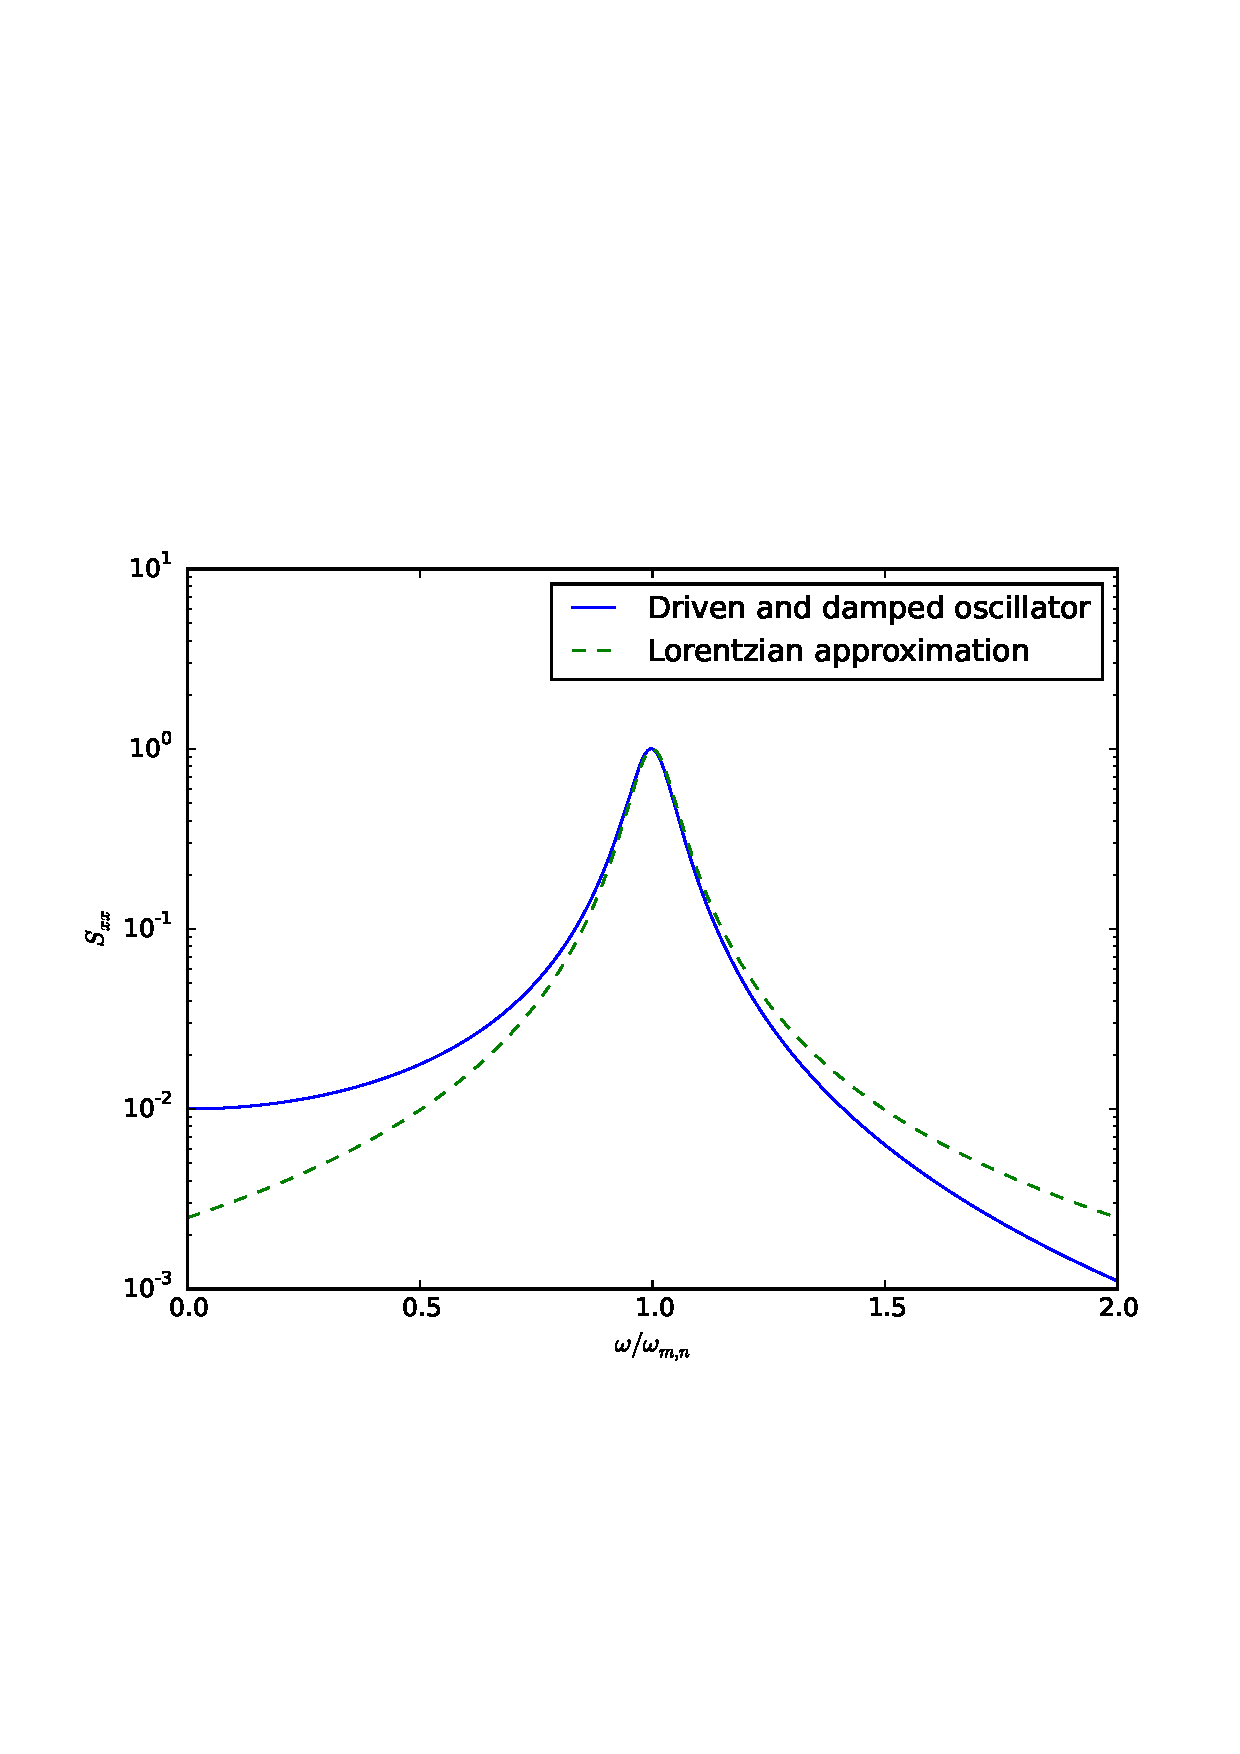
\includegraphics[scale=0.8]{lorentzian_approx.png}
\caption{Normalized power spectral density for arbitrary parameters of a mechanical oscillator (blue). The dashed (green) line is the Lorentzian approximation for the same parameters.}
\label{fig:lor_approx}
\end{figure}